\documentclass[12pt,letterpaper]{exam}
\usepackage[lmargin=1in,rmargin=1in,tmargin=1in,bmargin=1in]{geometry}
\usepackage{../style/exams}

% -------------------
% Course & Exam Information
% -------------------
\newcommand{\course}{MAT 108: Exam 3}
\renewcommand{\term}{Fall -- 2023}
\newcommand{\examdate}{12/14/2023}
\newcommand{\timelimit}{85 Minutes}

\setbool{hideans}{true} % Student: True; Instructor: False

% -------------------
% Content
% -------------------
\begin{document}

\examtitle
\instructions{Write your name on the appropriate line on the exam cover sheet. This exam contains \numpages\ pages (including this cover page) and \numquestions\ questions. Check that you have every page of the exam. Answer the questions in the spaces provided on the question sheets. Be sure to answer every part of each question and show all your work. If you run out of room for an answer, continue on the back of the page --- being sure to indicate the problem number.} 
\scores
\bottomline
\newpage

% ---------
% Questions
% ---------
\begin{questions}

% Question 1
\newpage
\question[10] Find the dual problem for the linear programming problem below. 
	\[
	\begin{gathered}
	\min w= 3y_1 - y_2 + 7y_3  \\
	\begin{cases}
	y_1 + y_2 + y_3 \geq 4 \\
	11y_1 + 15y_3 \geq 15 \\
	3y_1 + y_2 - y_3 \geq -9 \\
	8y_1 - 6y_2 + y_3 \leq 19 \\
	y_1, y_2, y_3 \geq 0
	\end{cases}
	\end{gathered}
	\]



% Question 2
\newpage
\question[10] Define the following matrices and vectors:
	\[
	\mathbf{u}= \begin{pmatrix} -4 \\ 7 \\ 3 \end{pmatrix}, \quad 
	\mathbf{v}= \begin{pmatrix} -6 \\ 5 \\ -8 \end{pmatrix}, \quad
	A= \begin{pmatrix} 1 & 3 \\ 0 & -1 \\ 4 & 5 \end{pmatrix}, \quad 
	B= \begin{pmatrix} 6 & -1 & 5 \\ 2 & 3 & 1 \end{pmatrix}
	\]
Showing all work, compute the following:
	\begin{enumerate}[(a)]
	\item $-2\mathbf{v} + \mathbf{u}$
	\item $\mathbf{u} \cdot \mathbf{v}$
	\item $AB$
	\end{enumerate}



% Question 3
\newpage
\question[10] Find the augmented matrix associated to the system of linear equations below. 
	\[
	\begin{gathered}
	x - y + z= 26 \\
	2x + 3y - z= 8 \\
	13x + 24y= 96
	\end{gathered}
	\]



% Question 4
\newpage
\question[10] Below is the final simplex tableau for a linear programming maximization problem. \par
	\begin{table}[H]
	\centering
	\begin{tabular}{cccccccccr}
	$48.33$ & $38.09$ & $0$ & $0$ & $21.89$ & $1$ & $-0.52$ & $0$ & $0.58$ & $569.24$ \\
	$0.2$ & $0.12$ & $0$ & $1$ & $0.08$ & $0$ & $0.02$ & $0$ & $0$ & $7.28$ \\
	$38.63$ & $10.73$ & $0$ & $0$ & $20.46$ & $0$ & $-0.07$ & $1$ & $-0.63$ & $257.45$ \\
	$0.23$ & $0.34$ & $1$ & $0$ & $0.56$ & $0$ & $-0.01$ & $0$ & $0.02$ & $5.54$ \\
	$2.5$ & $10.23$ & $0$ & $0$ & $14.52$ & $0$ & $0.1$ & $0$ & $0.13$ & $131.02$
	\end{tabular}
	\end{table} \par

\begin{enumerate}[(a)]
\item How many inequalities were considered?
\item How many variables were there in the original inequalities?
\item How many slack/surplus variables were introduced?
\item What was the solution to this maximization problem?
\end{enumerate}



% Question 5
\newpage
\question[10] The following matrix is the RREF of an augmented matrix coming from a system of equations. Did this system of equations have a solution? If the system of equations had a solution, find all the possible solutions. If the system did not have a solution, explain why. 
	\[
	\begin{pmatrix}
	1 & 0 & 0 & 0 & 0 & 0 \\
	0 & 1 & 0 & 0 & 0 & 67.5 \\
	0 & 0 & 1 & 0 & 0 & -46.7 \\
	0 & 0 & 0 & 1 & 0 & 51.2 \\
	0 & 0 & 0 & 0 & 1 & 0 
	\end{pmatrix}
	\]



% Question 6
\newpage
\question[10] Find the initial simplex tableau for the linear programming below. 
	\[
	\begin{gathered}
	\hspace{-1cm} \max z= 3x_1 - 5x_2 + 9x_3 \\
	\begin{cases}
	x_1 + 2x_2 - x_3 \leq 12 \\
	5x_1 + 19x_2 \leq 45 \\
	4x_1 - 5x_2 + 5x_3 \geq 27 \\
	-7x_1 - 6x_2 + 6x_3 \leq -12 \\
	x_1, x_2, x_3 \geq 0
	\end{cases}
	\end{gathered}
	\]



% Question 7
\newpage
\question[10] The following matrix is the RREF of an augmented matrix coming from a system of equations. Did this system of equations have a solution? If the system of equations had a solution, find all the possible solutions. If the system did not have a solution, explain why. 
	\[
	\begin{pmatrix}
	1 & 0 & 0 & 3 \\
	0 & 1 & 0 & -7 \\
	0 & 0 & 0 & 1 
	\end{pmatrix}
	\]



% Question 8
\newpage
\question[10] Below is the initial simplex tableau corresponding to a linear programming maximization problem. Find the initial maximization problem. \par
	\begin{table}[H]
	\centering
	\begin{tabular}{rrrrrr}
	$-5$ & $6$ & $1$ & $0$ & $0$ & $12$ \\
	$1$ & $1$ & $0$ & $-1$ & $0$ & $3$ \\
	$3$ & $-2$ & $0$ & $0$ & $1$ & $19$ \\
	$-6$ & $5$ & $0$ & $0$ & $0$ & $0$ 
	\end{tabular}
	\end{table} \pspace



% Question 9
\newpage
\question[10] The following matrix is the RREF of an augmented matrix coming from a system of equations. Did this system of equations have a solution? If the system of equations had a solution, find all the possible solutions. If the system did not have a solution, explain why. 
	\[
	\begin{pmatrix}
	1 & 0 & 0 & 12 \\
	0 & 1 & -4 & 15 \\
	0 & 0 & 0 & 0 
	\end{pmatrix}
	\]



% Question 10
\newpage
\question[10] Researchers are trying to determine the relationship between age, $a$, and Christmas spirit, $S$. They asked 180 individuals aged 1 to 92 their level of Christmas spirit (on a scale of 0 -- 100). Given the scatterplot of the data, plotted below, they create a linear model for the data---also plotted below. The least square regression line was found to be $\widehat{S}(a)= 87.98 - 0.62a$ with $r= 0.956971$. \par
	\begin{figure}[h]
	\centering
	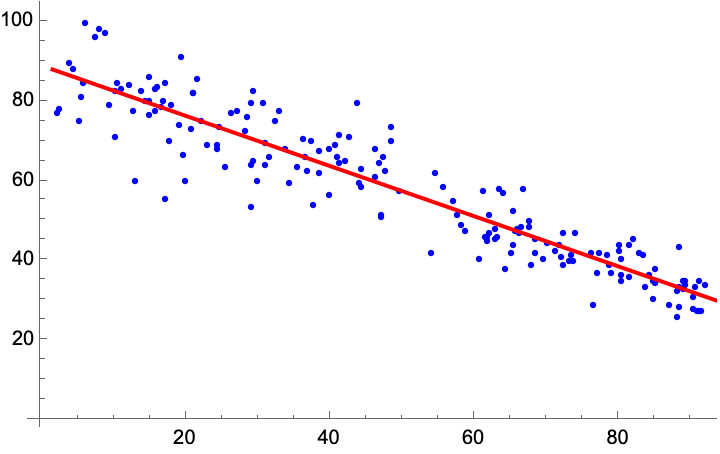
\includegraphics[width=0.45\textwidth]{xmas_spirit.png}
	\end{figure}

\begin{enumerate}[(a)]
\item Find $b_0$ and $b_1$ for this model. 
\item Was Christmas spirit positively or negatively correlated with age? Explain.
\item If a participant in this study, aged 29, rated their Christmas spirit as 62, find the residual for this individual. 
\item Find and interpret the coefficient of determination. 
\item Based on (d), is this a `good' linear model? Explain. 
\end{enumerate}
	

\end{questions}
\end{document}